\chapter{Concept}

    \paragraph{Into}
    \begin{enumerate}
        \item Classification approaches with surrogate model
        \item Define problems that related with surrogates model
        \item Ideas on how to solve it
        \item Discussion
    \end{enumerate}

    In this section general applicability of surrogate model presented. With different applicability use cases, there are some obstacles occurred that have a place to be in all circumstances.

    General problem trade-off is producing the best possible multi-objective solution with less effort. Because we consider expensive to the evaluation system, an effort first of all means really evaluated examples. Each of this evaluation can require a lot of time, energy or other resources. That is why the main comparison criteria for approach in solving the multi-objective problem is reducing the count of experiments. Moving further is a question: What does it mean, solving a multi-obj problem?
    \begin{itemize}
        \item Single-point, that is Pareto optimal solution
        \item Multi-point solutions that all is Pareto optimal
    \end{itemize}

    In this work under solving a multi-objective problem, we intend to find a set of none-dominated points that cover a wide range of objectives values and close to true Pareto front as possible. For reach, this goal multiple algorithms could be applied but MOEA is favoured choice. The advantage of evolutionary algorithms is that it could be easily modified. It operate on a set of solution candidates, that are well-fitted to approximate Pareto-front. Finally, it has been demonstrated in various usecases that evolutionary algorithms can estimate highly complex problems. With constrains as expensive evaluations, the real count of experiments could be reduced throw applying a multi-objective algorithm on a surrogate model. This technique is the preferred choice for functional optimization when the evaluation cost is large.

    As shown before for a black-box expensive problem suited surrogate or model-based optimization. But this approach also has open questions and limitations:
    \begin{itemize}
        \item Multi-objectivity. They are not too many surrogate models that can handle multi-dimensional objective space. Also scaling existing multi-output surrogate model is an open research question
        \item Surrogate is domain-specific. For improving and reach the best of the best prediction we should know in cross-grain basic objective surface to apply certain surrogate. Universal surrogates can gain optimal results but not the best possible
        \item Quality of prediction depends on how much samples do we have for a specific type of surrogate. There is additionally trade-off between reducing samples size and maximize the quality of prediction.
        \item Categorical features. A lot of real-world problems depends on the categorical feature. Parameter tuning with that type of space is not trivial
        \item Often Optimization algorithm and surrogate model are very tightly coupled. Highly united implementation can reduce the search possibility of algorithm and suitable for a specific type of problem. Reimplementing these algorithms for each usage scenario becomes timeconsuming and error-prone.
    \end{itemize}

    Mainly two groups are affected by this problem:
    \begin{itemize}
        \item Application engineers who need to choose, implement, and apply state-of-the-art algorithms without in-depth programming knowledge and expertise in the optimization domain
        \item Developers of optimization methods who want to evaluate algorithms on different test problems and compare a variety of competing methods
    \end{itemize}

    For slow computational problems, it would be useful to modulate a problem using a quite small number of most informative examples. This general topic introduces compositional surrogate, as a proxy model that approximate objectives surfaces and support MOEA to evaluates near a multi-objective solution and predict better multi-objective samples on each iteration.


    There is a clear need for a method to provide and distribute ready-to-use implementations of optimization methods and ready-to-use benchmark and real-world problems. 
    These modules should be freely combinable. Since the above- mentioned issues are not constrained to evolutionary optimization a candidate surrogates solution should be applicable to a broader range of search algorithms.

    The main objective of this part is to provide a thorough treatment of multi-objective parameter tuning with evolutionary algorithm(s)

    Key description how to improve solutions for problems in research questions.

    Multi-objective optimizations are frequently encountered in engineering practices. The solution techniques and parametric selections however are usually problem-specific. \cite{abs181207958}

    % --------------------------------------------------------------------------------------------
    % ------------------------------------------------     Compositional Surrogate model      
    % --------------------------------------------------------------------------------------------
    \section{Compositional Surrogate Model}

        The potential for applying surrogate is laid in the fast evaluation of the surrogate model. This advantage should outperform disadvantage in time required to build this surrogate model. In classical model-based optimization is used single surrogate-model that provide a hypothesis on the relation between parameter and objective space. There is a lot type of models that can do it but out and away fewer models that can manage multidimensionality objective space. The perspective way to create multi-objective surrogate is stacking multiple simple models into one that describes complex objective space. Notwithstanding that those models could be completely different and build in parallel, they still related because fitted on intersection features.
        Splitting optimization problem to multiple stages improves the reusability of code and makes approach scalable. Nevertheless, we can switch from single-obj to multi obj and change optimization technic on the fly.


        \begin{figure}
            \centering
            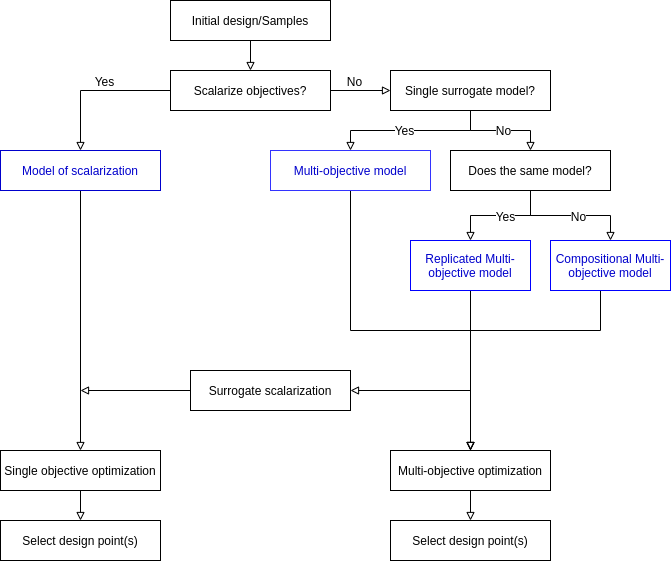
\includegraphics[width=\textwidth]{content/images/mbmo.png}
            \caption[Generalized MBMO algorithm]{Generalized MBMO algorithm}
            \label{fig:generalMBMO}
        \end{figure}


        A surrogate model is either selected randomly or due to its popularity in the area with which the problem is associated.  However, there are still some open challenges related to the ensemble of meta- models such as what should be the criterion for choosing different metamodels or how different metamodels can be used simultaneously? In addition, there are no guidelines for using different models for different objective functions \cite{SoftSurvey}.

    % --------------------------------------------------------------------------------------------
    % ------------------------------------------------     Domain-specific Surrogate model      
    % --------------------------------------------------------------------------------------------
    \section{Domain-specific problem}
    With gain to find the best solution with less effort surrogate models is domain-specific. It's mean that from two surrogate models in two different problems the best surrogate is changing. It could interpreter as Non-free lunch theorem in model-based optimization. If we extend this argument then the same optimization problem in different parameter tuning iteration could be interpreted as another optimization problem. This means that to reduce effort and increase the convergence of an algorithm we should change the surrogate model depend on how much samples do we have. As one would expect, no approximation method is universal.
    This leads us to use a portfolio with surrogate models. As a negative consequence, the model fitting additional introduces an additional overhead into the optimization.
    

    % --------------------------------------------------------------------------------------------
    % ------------------------------------------------     Surrogate Validation      
    % --------------------------------------------------------------------------------------------
    \section{Surrogate Validation}
    It is necessary to sacrifice a small portion of the data experiments to check the quality of the surrogate model on it. Based on validation results we can discard inadequate models and in a complex manner evaluated quality of solutions from valid models. If neither model is valid, this means that the best solution right now is a random solution. This may be due to insufficiently count of samples for the model or incorrect surrogate model, which is unable to describe the hypothesis between the configuration and objective space. 
    In the context of parameter tuning a common misconception is that we are interested in the accuracy of the model not in the entire space but in the optimal region. That is why evaluation surrogate validity based only on the coefficient of determination(R2) metrics is incorrect. Global R2 can be anyway used as a threshold in which if the models score becomes smaller of some threshold value it is not valid even without further estimations. 


    % --------------------------------------------------------------------------------------------
    % ------------------------------------------------     Categorical parameters      
    % --------------------------------------------------------------------------------------------
    \section{Real parameters for optimization}
    Parameter tuning is not a trivial task. Coding features for a surrogate model can transform es in mining full form, understandable for a surrogate model. Encoding just represents a feature in another form that help model instanciation relation and a correlation between features. Based on this inner interpretation model can predict the values of labels based on a parameter vector. The problem occurs what we use the model as black-box to find a minimum of prediction and make reverse interpretation of this optimal predictions in the context of parameter space. Offen this prediction is not a feasible point from parameters space. As a possible solution, it partly transforms problem in multiple classification tasks and then considers there relation as a continuous problem for optimization [TPE]. For general surrogate model with mixed parameters, we can solve problem orthogonally with multiple optimizers. All categorical feature are encoded and with other numerical parameters were fitted to the surrogate model. Then we use this model as a source that describes the function of the mapping parameter to objective space.  We incrementally solve this optimization problem on a subset of dimension iteratively. For example, we find optimal parameters in categorical dimensions and then fix these values and optimize surrogate on the left sub set of numerical dimensions where categories are fixed.


    % --------------------------------------------------------------------------------------------
    % -----------------------------------------------------       Discussion      ----------------
    % --------------------------------------------------------------------------------------------
    \section{Discussion}

        % -----------------------------------------------------       Infill criteria       ------
        \paragraph{}{Infill criteria}
        In the case of MOEA, solution of algorithm present as non-dominated final population. Based on unbiased, multi-objective criteria, they all uniformly could be presented as a prediction to the next evaluation. They represents current solution based on the surrogate model. Nevertheless, there is prior knowledge available in samples which can be taken into account. To reduce the number of candidates in the population, it is possible to deny those in which the distance to the nearest available sample is less than their average distance.
        So there are two strategies for predicting from a population:
        \begin{itemize}
            \item Prior and posterior knowledge. Based on changing metrics in available and proposed solutions
            \item Posterior knowledge. Proposed solutions are all equal
        \end{itemize}


        
        % -----------------------------------------------------       Conclusions       ------
        Also, to the best of our knowledge, has not been previously or stingy reported in the efficient multi-objective optimization.
        Contribution:
        \begin{itemize}
            \item Surrogate combination/composition. Current approaches use the same model for each dimensionality
            \item Surrogate portfolio. Search a better hypothesis  for a specific problem at a particular stage of parameter tuning
            \item Metric combination for evaluation Pareto optimal points
            \item Samples size depends on model(s) validity
            \item Combination of different(orthogonal) solvers
        \end{itemize}

        Some of the major findings were \cite{SoftSurvey}:
        \begin{enumerate}
            \item Kriging and neural networks were the most commonly used surrogate models
            \item Most of the algorithms were based on dominance-based evolutionary algorithms
            \item Most of the algorithms solved the problems with no more than three objectives
            \item The number of decision variables was also limited especially when using Kriging
            \item Only few algorithms used an ensemble of metamodels 
            \item Many algorithms were tested only on benchmark problems which were not at all computationally expensive
        \end{enumerate}